%% quantum's style

\documentclass[a4paper,twocolumn,11pt]{quantumarticle}

\pdfoutput=1
\usepackage[utf8]{inputenc}
\usepackage[english]{babel}
\usepackage[T1]{fontenc}
\usepackage{amsmath}
\usepackage{hyperref}
%
%\usepackage{tikz}
%\usepackage{lipsum}


%% our previous style and packages

%\documentclass[two column]{article}
%\usepackage[utf8]{inputenc}
\usepackage{graphicx}
\usepackage[dvipsnames]{xcolor}
%\usepackage[colorlinks=true,linkcolor=Blue,hypertexnames=false]{hyperref}
\usepackage{braket}
\usepackage{bbold}



\usepackage[numbers,sort&compress]{natbib}
%\usepackage[style=phys]{biblatex}
\usepackage{amssymb}
%\usepackage{amsmath}
\usepackage{placeins}
\usepackage{subcaption}

\usepackage[left=23mm,right=23mm,top=35mm,columnsep=15pt]{geometry}

\usepackage{pgfplotstable}
\usepackage{array}

\usepackage[qm]{qcircuit}

\newcommand{\caro}[1]{\textcolor{red}{[#1]}}
\newcommand{\jovan}[1]{\textcolor{blue}{[#1]}}
\newcommand{\steve}[1]{\textcolor{purple}{[#1]}}




\title{Notes on $\mathbb{Z}_2$-SPT preparation protocols}
\author{Jovan Jovanovi\'c}
\affiliation{Rudolf Peierls Centre for Theoretical Physics, Parks Road, Oxford, OX1 3PU, UK}
\orcid{0000-0002-2508-3207}
\author{Carolin Wille}
\affiliation{Rudolf Peierls Centre for Theoretical Physics, Parks Road, Oxford, OX1 3PU, UK}
\orcid{0000-0002-9764-6937}
\author{Steven H. Simon}
\affiliation{Rudolf Peierls Centre for Theoretical Physics, Parks Road, Oxford, OX1 3PU, UK}
\orcid{0000-0001-7757-5978}



\date{11.08.2023.}

\begin{document}

\maketitle
\begin{abstract}
TBC  
\end{abstract}
\tableofcontents



\section{Overview}

Symmetry protected topological phases (SPTs) can be characterised by the properties of their fixed point wave-functions. Those properties are: \begin{enumerate}
\item Symmetric under an onsite representation of some symmetry group $G$.
\item It's parent Hamiltonian is gapped and it's ground state is unique, if the system lives on a closed manifold.
\item  If the manifold has an edge, a suitable parent Hamiltonian either supports a gapless edge mode or symmetry is spontaneously broken at the edge.
\end{enumerate}

Given the onsite symmetry group $G$ in $2+1$ dimensions we can classify all bosonic SPTs by the third cohomology group $\mathcal{H}^{3}(G, U(1))$ \cite{spt_coho_org}. Bosonic in this sense means that the elementary degrees of freedom commute, i.e. spin lattices. 

Given an element of the cohomology group $[\omega] \in \mathcal{H}^{3}(G, U(1))$ we can construct the fixed point wavefunction on a closed manifold.

For the case of concreteness we will immediately limit ourselves to the case at hand, $G = \mathbb{Z}_2$, its third cohomology group is $\mathcal{H}^{3}(\mathbb{Z}_2, U(1)) = \mathbb{Z}_2$. The two elements of the cohomology group represent the trivial paramagnet $\ket{\Psi_0}$ and our target state (the nontrivial SPT) $\ket{\Psi_1}$.

The two states are deceptively similar, given a spin-$1/2$ configuration on any lattice of $N$ sites the two states are: \begin{gather}
\ket{\Psi_0} = \sum_{\{s_i\}\in\{0,1\}^N}\ket{\{s_i\}}, \\ \ket{\Psi_1} = \sum_{\{s_i\}\in\{0,1\}^N}(-1)^{N_{d.w.}(\{s_i\})}\ket{\{s_i\}},
\end{gather} where $N_{d.w.}(\{s_i\})$ is the number of domain walls in a given configuration $\{s_i\}$. It is in the definition of this quantity that the embedding manifold plays a role.

\subsection{The fixed point Hamiltonian}

\section{State preparation on manifolds without boundary}

We will introduce our lattice, see Figure \ref{fig:3x3pbc} for an example,
\begin{figure}
\centering
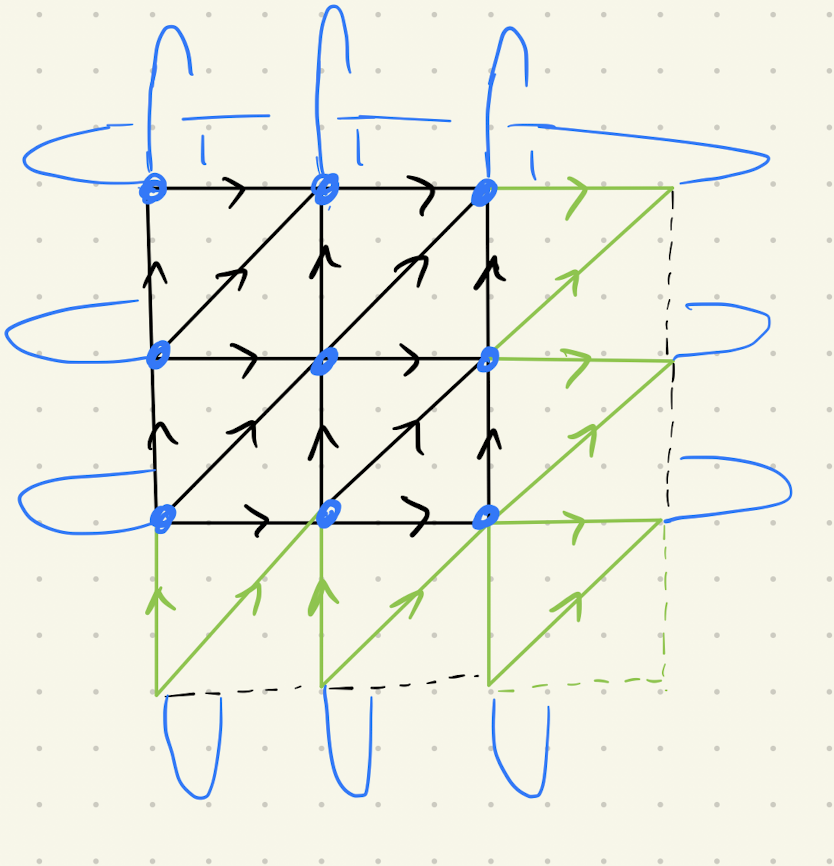
\includegraphics[width=\linewidth]{Figures/3x3_pbc.png}
\caption{An example of a N = 9 triangular lattice on a torus. (Proto)}
\label{fig:3x3pbc}
\end{figure}
in this example we have $N = 9$ spins on vertices of a triangular lattice on the periodic topology of a torus. For the sake of clarity we will drop the diagonal edges so we work with a simpler square lattice, only invoking the original stricture to resolve some ambiguities when it comes to defining $N_{d.w.}$ on a square lattice.

Given the simple structure of SPT states on closed manifolds, it is no surprise that there exist an efficient preparation protocol. In fact, once we prepare the trivial paramagnet we can just apply a phase to each plaquette according to a set of local plaquette rules, see Figure \ref{fig:plaq}.\begin{figure}
\centering
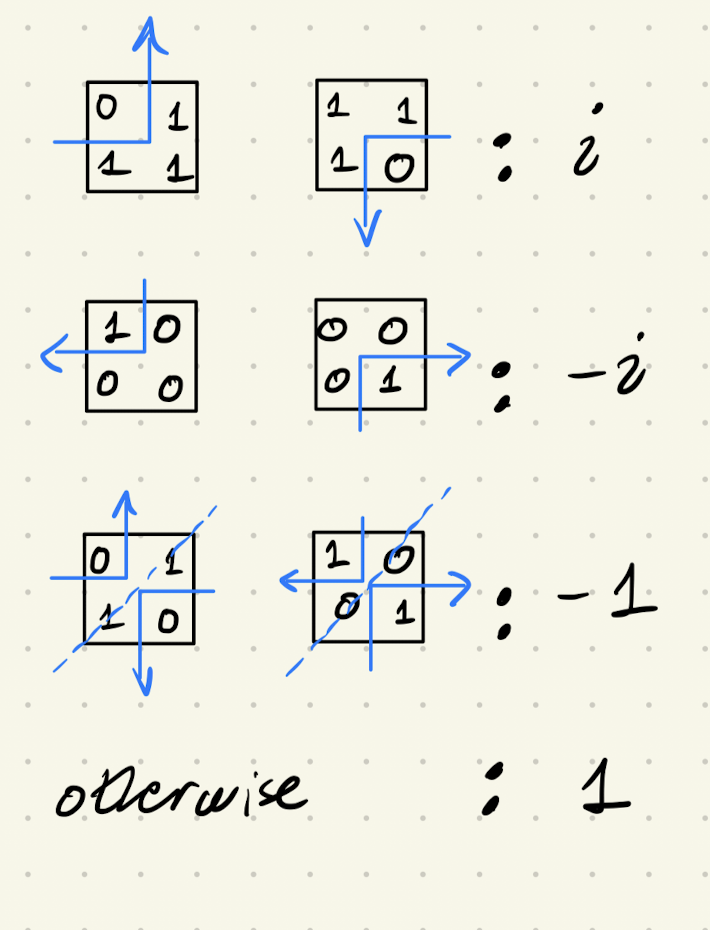
\includegraphics[width=\linewidth]{Figures/plaq_rules.png}
\caption{A set of plaquette rules that generate the correct phase factor on a closed manifold. (Proto)}
\label{fig:plaq}
\end{figure}
To see this generates the correct phase, consider the case of one rectangular domain. It contributes with the phase $i \times i =  - 1$ ($-i \times -i =  - 1$) due to its two out of four corners contributing the adequate phase. Furthermore, introducing kinks and elongating the wall doesn't change the overall phase associated with that domain wall. Note that the rules are not compatible with the symmetries of the square precisely because the underlying structure is a triangular lattice.

It is also imperative to emphasise that these rules only reproduce the correct phase if we deal with a regular square lattice on a torus.
This, however, is far form the unique set of local rules. They are many that reproduce the same phase on a closed manifold, however thet all fail if the manifold has an edge (where domain walls enter and leave the system without closing).

\emph{Concrete protocol.} We will describe the concrete protocol for preparing a SPT fixed point wavefunction on a regular cubic lattice on a torus. 

Given the following layout of qubit's on the chip, see Figure \ref{fig:chip},
\begin{figure}
\centering
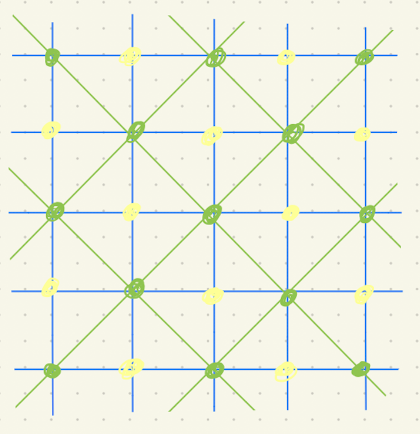
\includegraphics[width=\linewidth]{Figures/on_chip.png}
\caption{The layout of cubits on the chip. The green qubits represent the spin-1/2 physical degrees of freedom, while the yellow qubits (one per green plaquette) are used as auxiliary degrees of freedom. The blue links are representing the physical links between qubits on the chip over which we can implement two-qubit gates.}
\label{fig:chip}
\end{figure}
the protocol can be formulated in following six steps, see Figure \ref{fig:prot}.
\begin{figure}
\centering
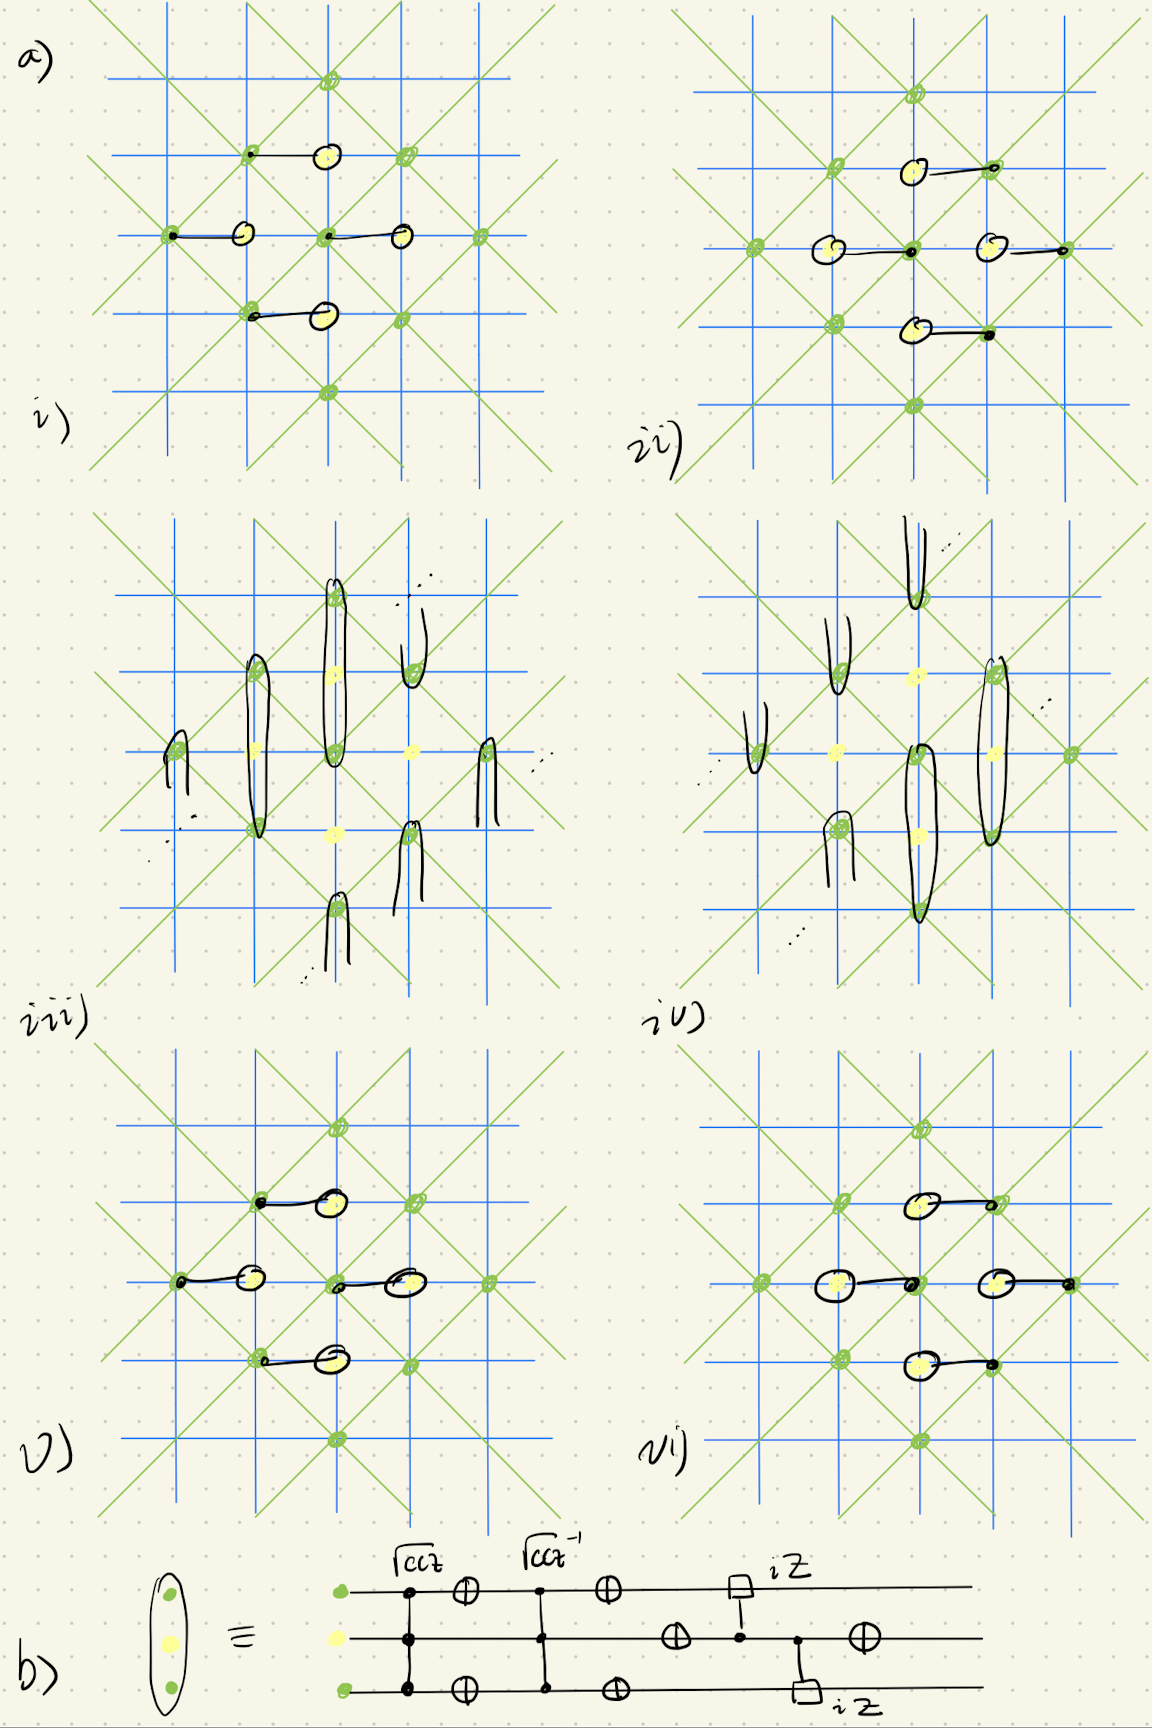
\includegraphics[width=\linewidth]{Figures/torus_protocol.png}
\caption{The six step protocol for preparing the $\mathbb{Z}_2$-SPT fixed point wavefunction on a regular square lattice on a torus.}
\label{fig:prot}
\end{figure}

The six steps are as follows:\begin{enumerate}
\item Given all states start in the state $\ket{0}$ apply a Haddamard gate to all green qubits (not shown in Figure \ref{fig:prot}),
\item Apply a CNOT gate from each green qubit to the auxiliary qubit to its left (Figure \ref{fig:prot}a.i.),
\item Apply a CNOT gate from each green qubit to the auxiliary qubit to its right (Figure \ref{fig:prot}a.ii.),
\item Apply the three-qubit circuit shown in Figure \ref{fig:prot}b. to the triples shown in Figure \ref{fig:prot}a.iii. implementing the local plaquette phase rules on the plaquettes in the odd rows,
\item Apply the three-qubit circuit shown in Figure \ref{fig:prot}b. to the triples shown in Figure \ref{fig:prot}a.iv. implementing the local plaquette phase rules on the plaquettes in the even rows,
\item Repeat steps 1. and 2. to disentangle the auxiliary qubits.
\end{enumerate}



%\printbibliography

\bibliographystyle{quantum}
\bibliography{bibliography}

\end{document}
